\documentclass{article}

\usepackage{graphicx}
\usepackage{tikz}
\usepackage{tikzsymbols}
\usetikzlibrary{calc,patterns,shapes.geometric}
\pagestyle{empty}
\usepackage[margin=0pt]{geometry}
\geometry{papersize={14in,12in}}

\def\centerarc[#1](#2)(#3:#4:#5){\draw[#1] ($(#2)+({#5*cos(#3)},{#5*sin(#3)})$) arc (#3:#4:#5);}

\begin{document}
	\begin{figure}
		\centering
		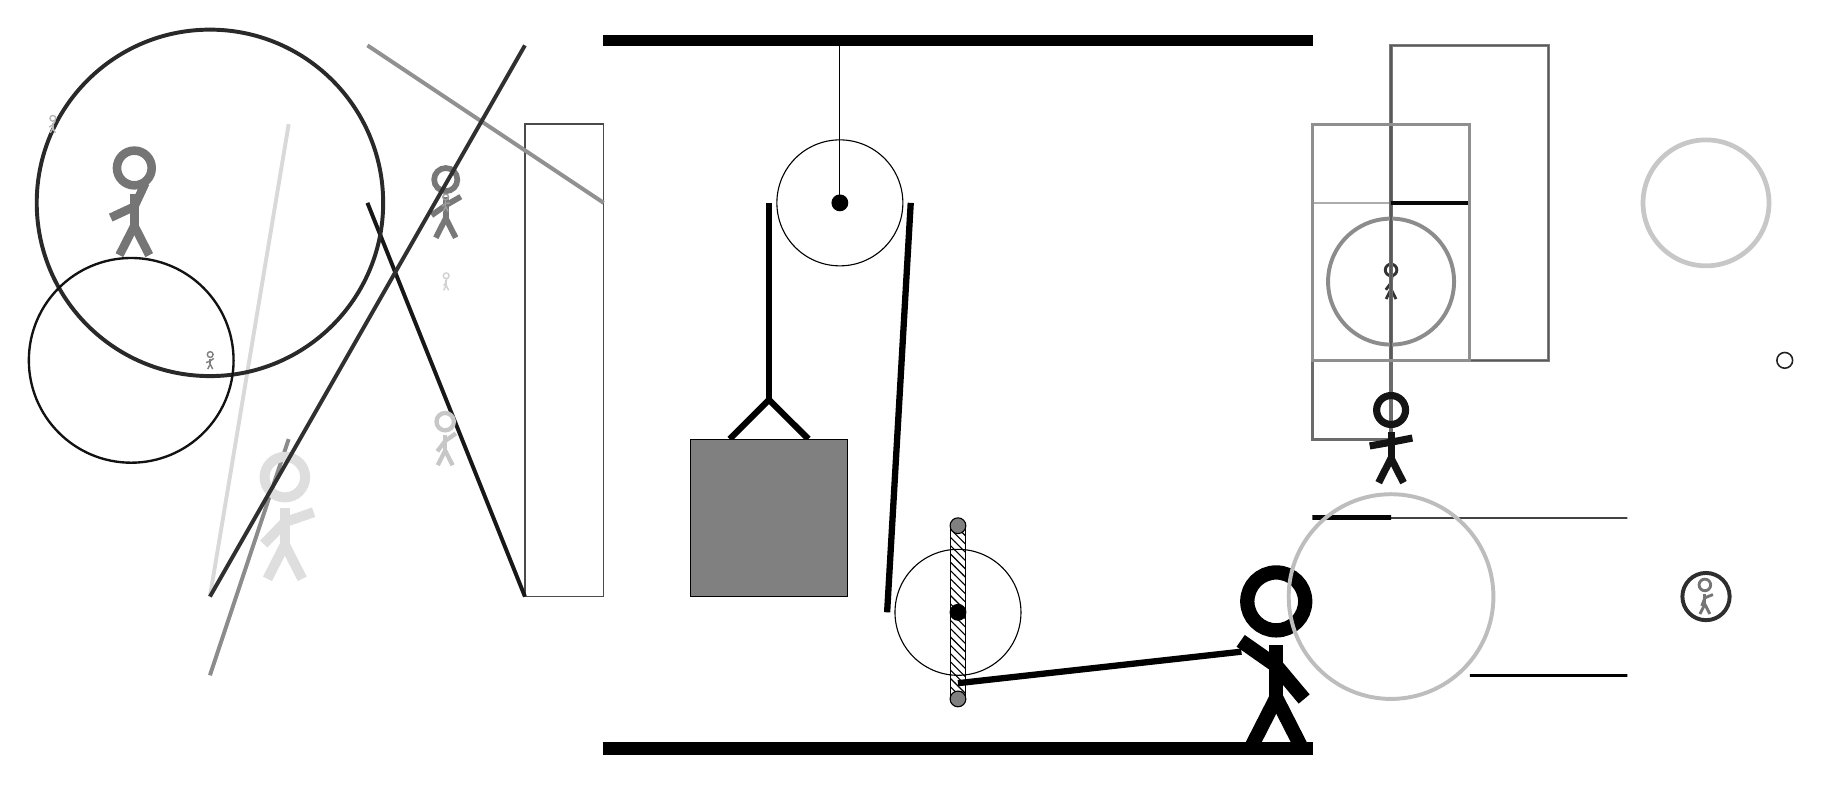
\begin{tikzpicture}
			%%%%% START %%%%%
			
			\draw[fill=black] (-2, 9) rectangle (7, 9.125);
			
			\draw (1, 7) circle (0.8);
			\draw[fill=black] (1, 7) circle (0.1);
			\draw (1, 9) -- (1, 7);
			
			\draw[fill=white](2.5, 1.8) circle (0.8);
			\draw[fill=black] (2.5, 1.8) circle (0.1);
			\draw[pattern=north west lines, pattern color=black] (2.4, 2.9) rectangle (2.6, 0.7);
			\draw[fill=black!50] (2.5, 2.9) circle (0.1);
			\draw[fill=black!50] (2.5, 0.7) circle (0.1);
			
			\draw[line width=0.8mm] (-0.4, 4.0) -- (0.1, 4.5) -- (0.6, 4.0);
			\draw[fill=black!50] (-0.9, 4.0) rectangle (1.1, 2.0);
			
			\draw[line width=0.8mm] (0.1, 7) -- (0.1, 4.5);
			\centerarc[line width=0.8mm](1, 7)(0:180:0.9);
			\draw[line width=0.8mm](1.9, 7) -- (1.6, 1.8);
			\centerarc[line width=0.8mm](2.5, 1.8)(180:270:0.9);
			\draw[line width=0.8mm](2.5, 0.9) -- (6.1, 1.3);
			
			\node at (6.5, 1.2) {\Strichmaxerl[10][-35][-50]};
			
			\draw[line width=0.5mm, color=black!45](-6, 4) -- (-7, 1);
			
			\draw[line width=0.4mm, color=black!100] (9, 1) rectangle (11, 1);
			\draw[line width=0.4mm, color=black!51] (8, 5) rectangle (10, 9);
			\node[line width=0.5mm, color=black!80] at (8, 6) {\Strichmaxerl[2][53][81]};
			
			\draw[line width=0.3mm, color=black!74] (8, 3) rectangle (11, 3);
			\draw[line width=0.3mm, color=black!32] (7, 5) rectangle (8, 7);
			\draw [line width=0.5mm, color=black!82](12, 2) circle (0.3);
			\draw[line width=0.5mm, color=black!15](-6, 8) -- (-7, 2);
			\draw[line width=0.2mm, color=black!71] (-2, 8) rectangle (-3, 2);
			\node[line width=0.7mm, color=black!18] at (-4, 6) {\Strichmaxerl[1][54][83]};
			\node[line width=0.6mm, color=black!53] at (-4, 7) {\Strichmaxerl[4][35][30]};
			
			\draw[line width=0.6mm, color=black!98] (7, 3) rectangle (8, 3);
			\node[line width=0.5mm, color=black!54] at (12, 2) {\Strichmaxerl[2][69][22]};
			\draw [line width=0.2mm, color=black!87](13, 5) circle (0.1);
			\draw[line width=0.4mm, color=black!58] (7, 8) rectangle (8, 4);
			\node[line width=0.3mm, color=black!54] at (-8, 7) {\Strichmaxerl[6][25][65]};
			\node[line width=0.3mm, color=black!92] at (8, 4) {\Strichmaxerl[5][10][11]};
			\node[line width=0.5mm, color=black!50] at (-7, 5) {\Strichmaxerl[1][22][36]};
			\draw[line width=0.5mm, color=black!91](-5, 7) -- (-3, 2);
			\draw[line width=0.5mm, color=black!43](-2, 7) -- (-5, 9);
			\draw [line width=0.5mm, color=black!45](8, 6) circle (0.8);
			
			\draw [line width=0.5mm, color=black!26](8, 2) circle (1.3);
			
			\draw[line width=0.2mm, color=black!65] (8, 9) rectangle (10, 5);
			\node[line width=0.2mm, color=black!13] at (-6, 3) {\Strichmaxerl[7][46][19]};
			\draw [line width=0.5mm, color=black!84](-7, 7) circle (2.2);
			\node[line width=0.3mm, color=black!28] at (-9, 8) {\Strichmaxerl[1][32][58]};
			\node[line width=0.6mm, color=black!22] at (-4, 4) {\Strichmaxerl[3][53][35]};
			\draw[line width=0.5mm, color=black!81](-7, 2) -- (-3, 9);
			\draw [line width=0.7mm, color=black!75](-4, 8) circle (0.0);
			\draw[line width=0.6mm, color=black!97] (8, 7) rectangle (9, 7);
			\node[line width=0.4mm, color=black!38] at (-4, 7) {\Strichmaxerl[1][40][7]};
			
			\draw [line width=0.6mm, color=black!22](12, 7) circle (0.8);
			\draw [line width=0.3mm, color=black!93](-8, 5) circle (1.3);
			
			\draw[line width=0.4mm, color=black!44] (9, 8) rectangle (7, 5);
			
			\draw[fill=black] (-2, 0) rectangle (7, 0.15);
			
			%%%%% END %%%%%
		\end{tikzpicture}
	\end{figure}	
\end{document}